\documentclass[a4paper,11pt]{article}
\usepackage[utf8]{inputenc}
\usepackage{amsfonts}
\usepackage{amsmath}
\usepackage{amssymb}
\usepackage{xcolor}
\usepackage{graphicx}
\usepackage[polish]{babel}
\usepackage[T1]{fontenc}
\usepackage{float}
\def\\{\hfill\break}


%----------------------
\title{Projekt Egzaminacyjny}
\author{Karol Krawczykiewicz, Piotr Maszczak}
\date{Listopad 2022 -- Styczeń 2023}

\begin{document}

\maketitle

\section{Wstęp}
Następująca analiza dotyczy dwóch spółek działających na rynku gier wideo
\\
\\
CD Projekt SA (CDR) - Grupa działa w dynamicznie rozwijającej się branży elektronicznej rozrywki. Opiera się na dwóch silnych fundamentach – produkcji gier w ramach studia deweloperskiego CD Project Red oraz globalnej cyfrowej dystrybucji realizowanej przez serwis GOG.com.
\\
\\
11 bit studios SA (11B) - Deweloper multiplatformowych gier sprzedawanych na całym świecie. Spółka zajmuje się każdym etapem tworzenia gier samodzielnie. Najbardziej znane gry to: Frostpunk i This War of Mine. Oprócz produkcji gier grupa zajmuje się również wydawaniem gier zewnętrznych oraz prowadzi internetową platformę sprzedaży.


\section {Analiza cen spółek}


\subsection{Spółka CD Projekt}




\begin{figure}[H]
    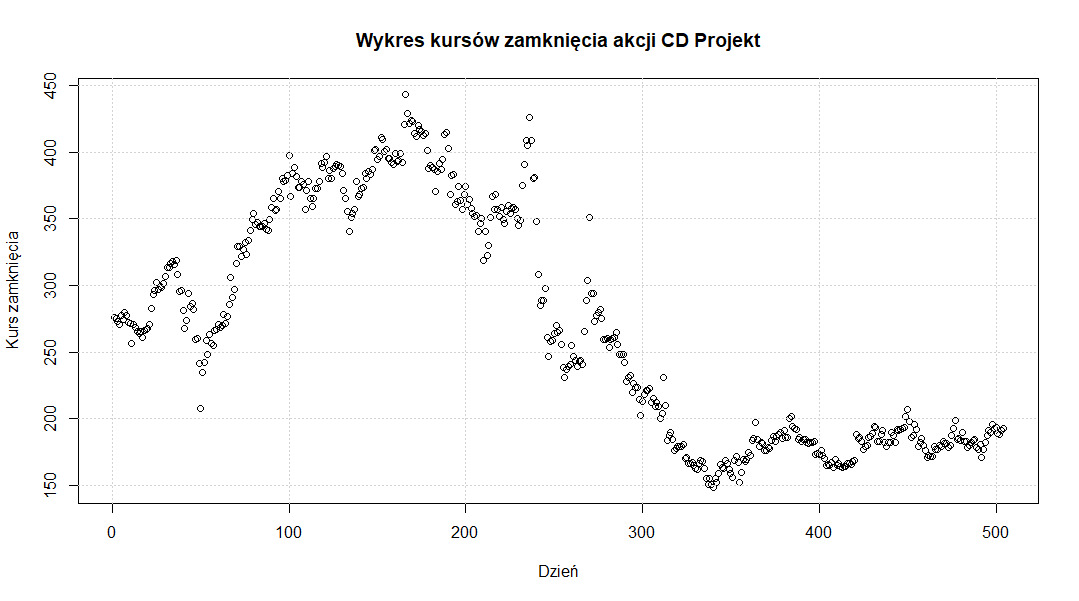
\includegraphics[width=13cm]{Wykresy CDR/CDR-kursy.png}
    \caption{Wykres akcji w przedziale czasowym od Stycznia 2020 do Grudnia 2021}
    \label{fig:mlp}
\end{figure}
\par
\\
\par
\begin{figure}[H]
    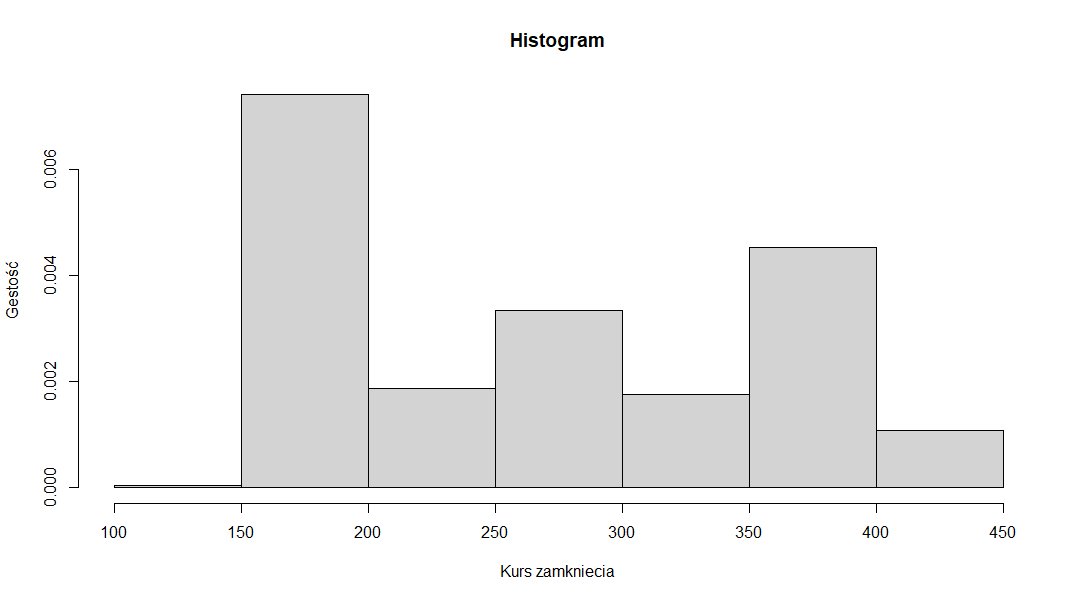
\includegraphics[width=13cm]{Wykresy CDR/CDR-histogram.png}
    \caption{Histogram gęstości}
    \label{fig:mlp}
\end{figure}


\par
\par
\begin{table}[H]
\centering 
\begin{tabular}{|l|l|l|l|l|}
\hline
      & \overline{x} & odch. st. & skośność  & kurtoza \\ \hline
Akcja & 277.6719           & 90.62922  & 0.2497853 & 1.56275 \\ \hline
\end{tabular}
\end{table}


Współczynnik skośności powyżej 0 świadczy o prawostronnej asymetrii rozkładu (wydłużone jest prawe ramię rozkładu). 
Kurtoza większa od 0 oznacza iż rozkład jest bardziej wysmukły niż normalny, większe skupienie wartości wokół średniej.

\\
\\
Wyestymowane parametry dla badanych rozkładów przy wykorzystaniu estymatora największej wiarygodności (MLE):
\begin{itemize}
  \item Rozkład normalny - mean 277.67190, sd 90.54032
  \item Rozkład log-normalny - meanlog 5.5719177, sdlog   0.3322444
  \item Rozkład gamma - shape 9.33484470 , rate  0.03362056
\end{itemize}

\begin{table}[H]
\centering 
\begin{tabular}{|l|l|l|l|l}
\cline{1-4}
                               & Normalny   & Log-normalny & Gamma      &  \\ \cline{1-4}
Kolmogorov-Smirnov statistic   & 0.1777046  & \colorbox{pink}{0.1715694}    & 0.1739537  &  \\ \cline{1-4}
Cramer-von Mises statistic     & 2.9612965  & 2.9246380    & \colorbox{pink}{2.8490879}  &  \\ \cline{1-4}
Anderson-Darling statistic     & 19.7989554 & 19.3686342   & \colorbox{pink}{19.1126404} &  \\ \cline{1-4}
Akaike's Information Criterion & 6047.228   & \colorbox{pink}{6010.751}     & 6013.699   &  \\ \cline{1-4}
Bayesian Information Criterion & 6055.697   & \colorbox{pink}{6019.220}     & 6022.168   &  \\ \cline{1-4}
\end{tabular}
\end{table}


Z powyższych danych wynika, iż rozkład Log-Normalny najlepiej opisuje kursy zamknięcia społki CDR. Trzy z pięciu przypadków optuje za rozkładem Log-Normalny, a dwa za rozkładem Gamma. 

\begin{figure}[H]
    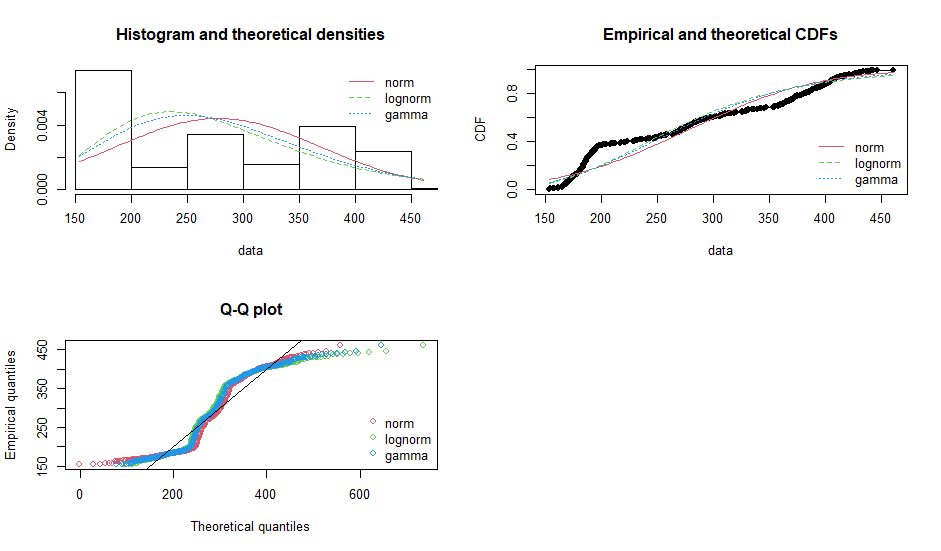
\includegraphics[width=13cm]{Wykresy CDR/CDP-estymatory.png}
    \caption{Wykresy diagnostyczne: Funkcje gęstości, Funkcja dystrybuanty, Kwantyle}
    \label{fig:mlp}
\end{figure}

Na podstawie wykresów diagnostycznych można wywnioskowac, że prawdopodbnie żaden z rozkładów nie będzie w dobrym stopniu odwzorowywał danych.




\centerline{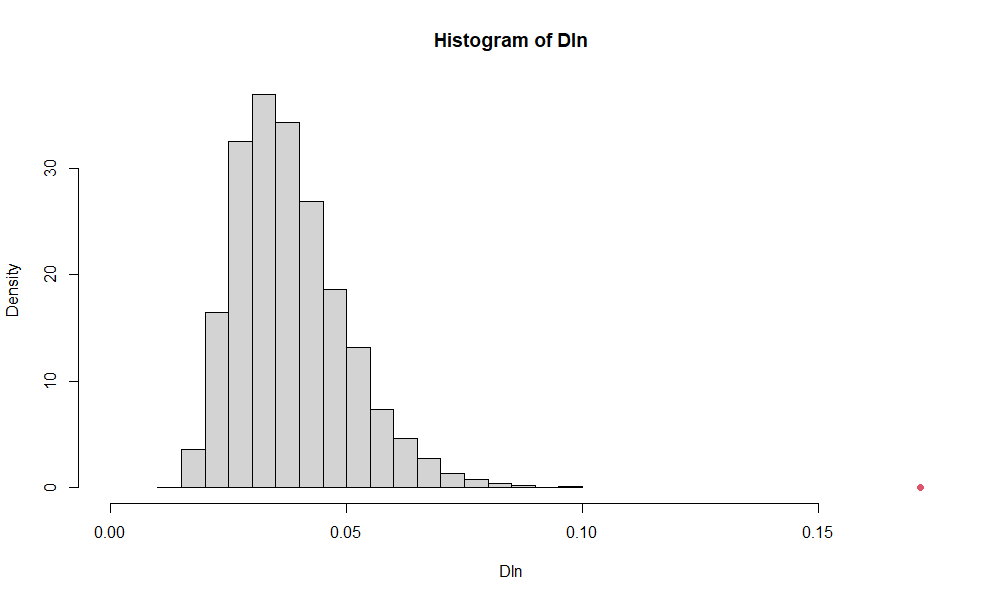
\includegraphics[width=13cm]{Wykresy CDR/CDP-MC.png}}

Po przetestowaniu hipotezy zerowej o równości dystrybuant, przy wykorzystaniu metody Monte-Carlo i statystyk Kołmogorowa-Smirnowa, uzyskano wyniki:
  $$ Dn = 0.1715694 $$
  $$p = length(Dn[Dn>dn])/N = 0$$ 
gdzie Dn to odleglość dystrybuant empirycznych od rozkładu logarytmiczno-normalnego, dn to wartość statystyki Dn, dla danych akcji spółki, N = 10000


\\
Wartość p jest mniejsza od przyjętego poziomu istotności,

   $$ \alpha  = 5\%$$

Zatem hipotezę o równosci dystrybuant odrzucamy.

%============================================================================================================
\subsection{Spółka 11 BIT STUDIOS}



\begin{figure}[H]
    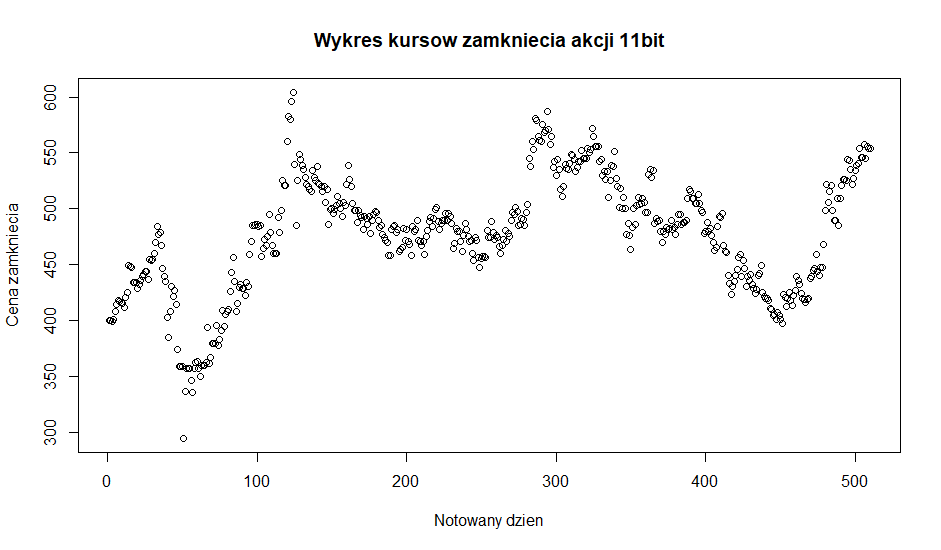
\includegraphics[width=13cm]{Wykresy 11B/11B-kursy.png}
    \caption{Wykres akcji w przedziale czasowym: Styczeń 2020 do Grudnia 2021}
    \label{fig:mlp}
\end{figure}
\par
\newpage
\par
\begin{figure}[H]
    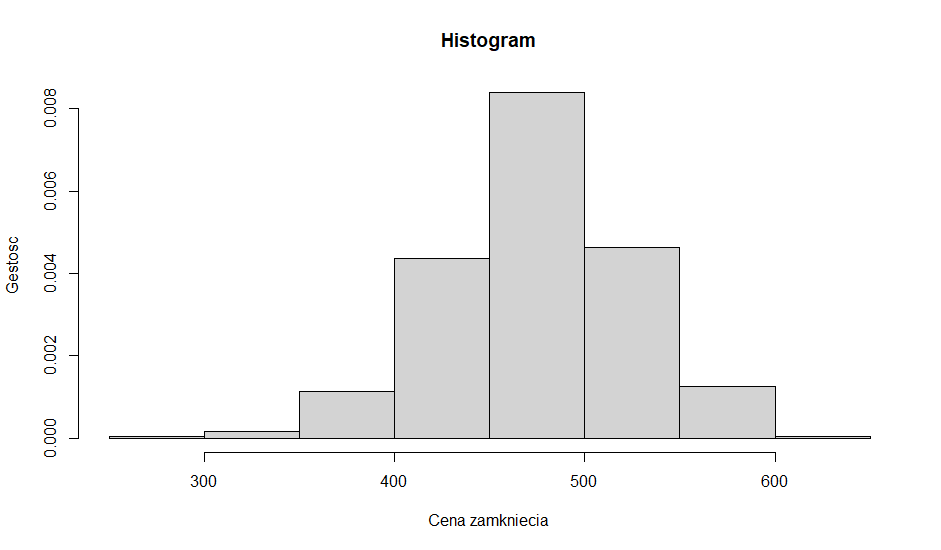
\includegraphics[width=13cm]{Wykresy 11B/11B-histogram.png}
    \caption{Histogram gęstości}
    \label{fig:mlp}
\end{figure}


\par
\par
\begin{table}[H]
\centering 
\begin{tabular}{|l|l|l|l|l|}
\hline
      & \overline{x} & odch. st. & skośność  & kurtoza \\ \hline
Akcja & 476.8853     & 51.16337  & -0.385939 & 3.071287 \\ \hline
\end{tabular}
\end{table}


Współczynnik skośności poniżej 0 świadczy o lewostronnej asymetrii rozkładu (wydłużone jest lewe ramię rozkładu). Kurtoza większa od 0 oznacza iż rozkład jest bardziej wysmukły niż normalny, większe skupienie wartości wokół średniej.

\\
\\
Wyestymowane parametry dla badanych rozkładów przy wykorzystaniu estymatora największej wiarygodności (MLE):
\begin{itemize}
  \item Rozkład normalny - mean 476.88529, sd 51.11319
  \item Rozkład log-normalny - meanlog 6.1612582, sdlog 0.1111746
  \item Rozkład Weibulla -  shape 10.73364, rate 499.28283
\end{itemize}

\begin{table}[H]
\centering 
\begin{tabular}{|l|l|l|l|l}
\cline{1-4}
                               & Normalny    & Log-normalny & Weibull      &  \\ \cline{1-4}
Kolmogorov-Smirnov statistic   & 0.06995126  & 0.0929663    & \colorbox{yellow}{0.06613342}  &  \\ \cline{1-4}
Cramer-von Mises statistic     & 0.38880200  & 0.7849020    & \colorbox{yellow}{0.30039685}  &  \\ \cline{1-4}
Anderson-Darling statistic     & 2.12780717  & 4.4814222    & \colorbox{yellow}{1.55241020} &  \\ \cline{1-4}
Akaike's Information Criterion & 5464.041    & 5495.215     & \colorbox{yellow}{5455.947}   &  \\ \cline{1-4}
Bayesian Information Criterion & 5472.510    & 5503.683     & \colorbox{yellow}{5464.416}   &  \\ \cline{1-4}
\end{tabular}
\end{table}


Z powyższych danych wynika, iż rozkład Weibulla najlepiej opisuje kursy zamknięcia społki 11 bit studios.
Wszystkie z pięciu przypadków wskazują za rozkładem Weibulla.

\begin{figure}[H]
    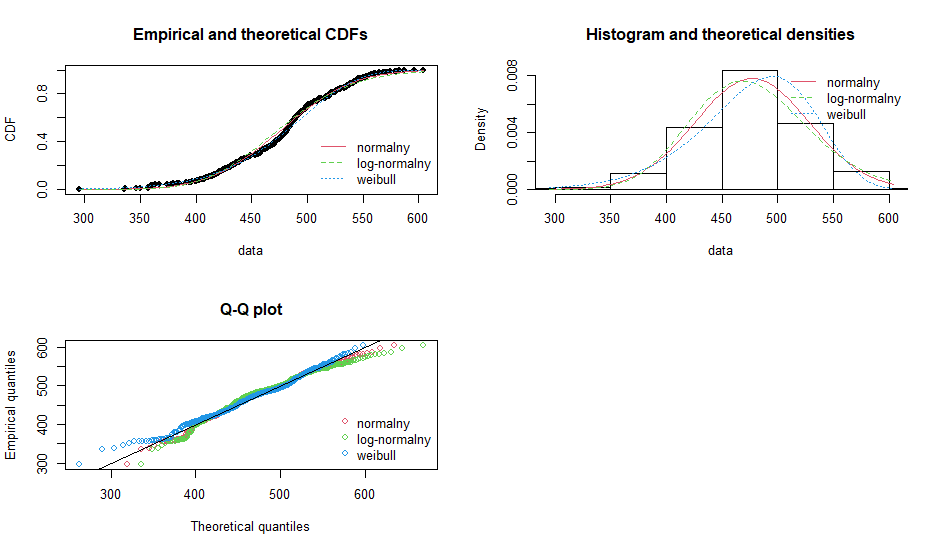
\includegraphics[width=13cm]{Wykresy 11B/11B-estymatory.png}
    \caption{Wykresy diagnostyczne: Funkcja dystrybuanty, Funkcje gęstości, Kwantyle}
    \label{fig:mlp}
\end{figure}

Na podstawie wykresów diagnostycznych można wywnioskować, że rozkład Weibulla najbardziej odwzorowuje dane.



\newpage
\centerline{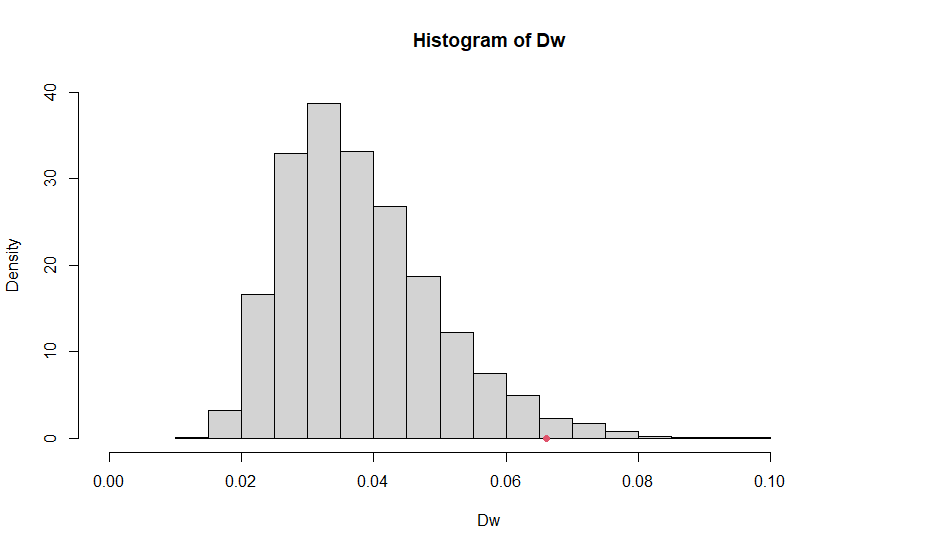
\includegraphics[width=13cm]{Wykresy 11B/11B-MC.png}}

Po przetestowaniu hipotezy zerowej o równości dystrybuant, przy wykorzystaniu metody Monte-Carlo i statystyk Kołmogorowa-Smirnowa, uzyskano wyniki:
  $$ Dw = 0.06613342 $$
  $$p = length(Dw[Dw>dw])/N = 0.0238$$ 

gdzie Dw to odleglość dystrybuant empirycznych od rozkładu Weibulla, dw to wartość statystyki Dw, dla danych akcji spółki, N = 10000

\\
Wartość p jest mniejsza od przyjętego poziomu istotności,

   $$ \alpha  = 5\%$$

Zatem hipotezę o równosci dystrybuant odrzucamy.





\newpage


\section{Analiza łącznego rozkładu log-zwrotów}
W tym rozdziale wykonujemy analizę dziennych log-zwrotów wcześniej wymienionych spółek: 11 bit studios oraz CD Projekt. 
\begin{figure}[H]
    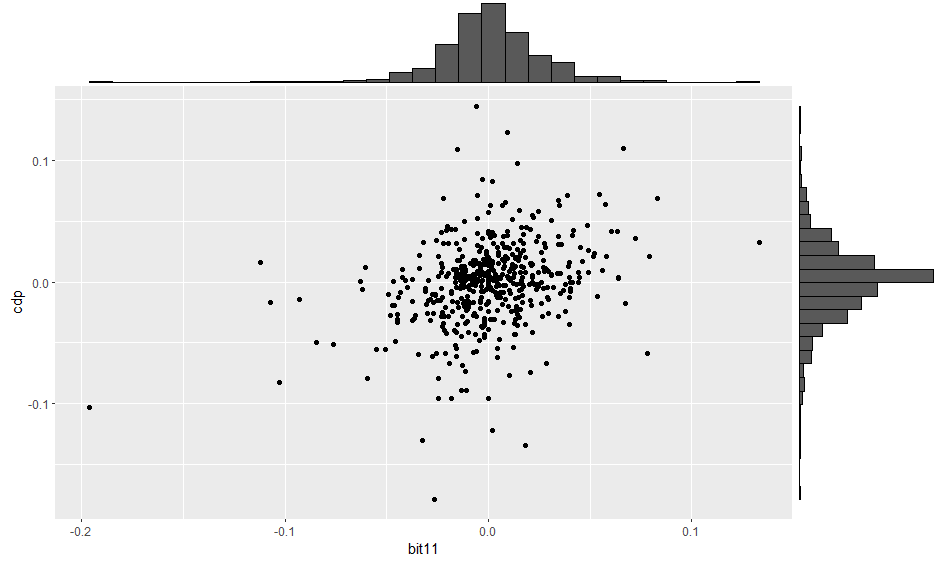
\includegraphics[width=13cm]{Wykresy/Histogram_rozkladow_brzegowych.png}
    \caption{Histogram rozkładów brzegowych}
    \label{fig:mlp}
\end{figure}
Z powyższego wykresu widać, że dane są znacznie rozproszone. Zauważalna częśc punktów skupia się wokół wektora średnich. Występuje tu dodatnia zależność. Duża ilość odstających wartości.
\begin{itemize}
  \item Wektor średnich $\hat{\mu}$ = (bit11: 0.000641, cdp: -0.00078)
  \item Kowariancja - cov 0.000311
  \item Współczynnik korelacji - cor 0.32332
\end{itemize} 

Wektor średnich $\hat{\mu}$ świadczy o średniej wartości poszczególnych zmiennych losowych. 

\\
Kowariancja jest bliska 0, oznacza to, że zmienne losowe nie są ze sobą związane w żaden szczególny sposób, istnieje słaby związek pomiędzy zmiennymi losowymi. W takim przypadku zmiany w jednej zmiennej nie są skorelowane z zmianami w drugiej zmiennej, nie występuje żadna zależność liniowa.

\\
Jeśli współczynnik korelacji wynosi 0.32, oznacza to, że istnieje słaba, dodatnia korelacja pomiędzy dwoma zmiennymi losowymi. To znaczy, że wzrost jednej zmiennej wiąże się z wzrostem drugiej zmiennej, ale związek ten nie jest silny. 

Wzór na macierz kowariancji: \\

\centerline{${\Sigma}$ = $\begin{bmatrix}
    Var(X) & cov(X,Y) \\
    cov(Y,X) & Var(Y)
\end{bmatrix}$ = 
$\begin{bmatrix}
    \sigma_1^2 & \rho\sigma_1\sigma_2 \\
    \rho\sigma_1\sigma_2 & \sigma_2^2
\end{bmatrix}$} \\
gdzie $\sigma_1$, $\sigma_2$ to odchylenia standardowe i $\rho$ współczynnik korelacji

\\
Macierz kowariancji dla analizowanych danych: \\
\begin{center}
    $\hat{\Sigma}$ = $\begin{bmatrix}
    0.00077 & 0.00031 \\
    0.00031 & 0.00117
\end{bmatrix}$
\end{center}\\

Wzór na macierz korelacji:  \\
$$\rho =
\begin{bmatrix}
1 & \frac{\text{cov}(X,Y)}{\sigma_X \sigma_Y} \\
\frac{\text{cov}(X,Y)}{\sigma_X \sigma_Y} & 1
\end{bmatrix}$$

\\
Macierz korelacji dla analizowanych danych: \\
\begin{center}
    $\begin{bmatrix}
    1 & 0.32332 \\
    0.32332 & 1
    \end{bmatrix}$
\end{center}


\begin{figure}[H]
    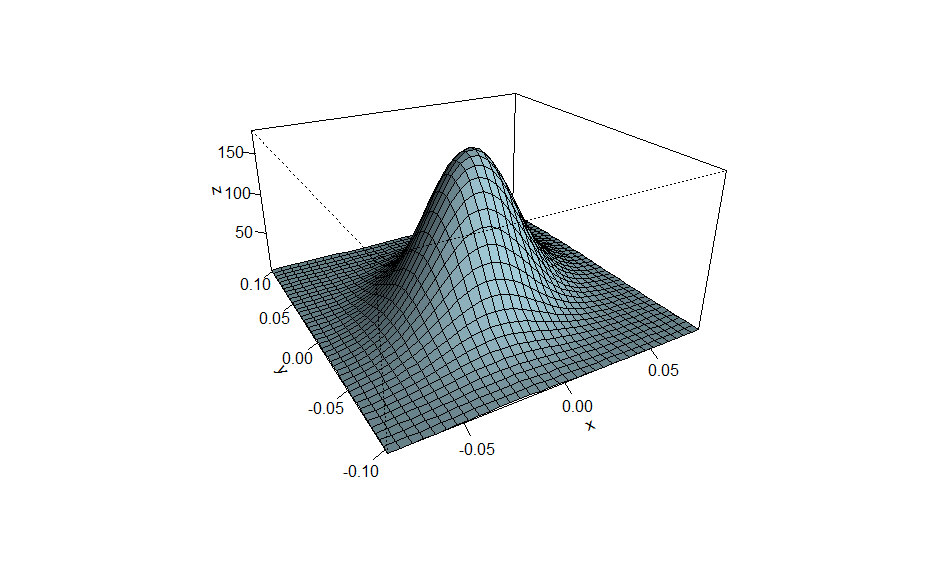
\includegraphics[width=13cm]{Wykresy/Wykres_gestosci.png}
    \caption{Wykres gęstości}
    \label{fig:mlp}
\end{figure}

\newpage

Gęstość rozkładu normalnego o wyestymowanych parametrach  jest zapisywana w następujący sposób:


$$f(x, y) = \frac{1}{2\pi\sigma_1\sigma_2\sqrt{1 - \rho^2}} \exp\left(-\frac{1}{2(1 - \rho^2)}\left[\frac{(x - \mu_1)^2}{\sigma_1^2} - 2\rho\frac{(x - \mu_1)(y - \mu_2)}{\sigma_1\sigma_2} + \frac{(y - \mu_2)^2}{\sigma_2^2}\right]\right)$$

gdzie $x$ i $y$ sa wektorami zmiennych losowych, $\hat{\mu}$ jest wektorem średnich, $\sigma_1$, $\sigma_2$ to odchylenia standardowe i $\rho$ współczynnik korelacji.\\
\\
Gęstość rozkładu normalnego dla analizowanych danych:

$$f(x, y) = 177.23\cdot\exp(-725.15(x-0.00064)^2 + 380.07(x-0.00064)(y+0.00078)$$
$$-477.24(y + 0.00078)^2)$$


\\
Gęstość rozkładów brzegowych jest zapisywana w następujący sposób:


$$f(x) = \frac{1}{\sigma\sqrt{2\pi}}\exp\left(-\frac{(x-\mu)^2}{2\sigma^2}\right)$$

\\

Gęstość rozkładów brzegowych dla analizowanych danych:


$$f_{11b}(x) = 14.39388\cdot\exp\left(-\frac{(x-0.00064)^2}{0.00154}\right)$$


$$f_{cdr}(x) = 11.65201\cdot\exp\left(-\frac{(x+0.00078)^2}{0.00234}\right)$$


\begin{figure}[H]
    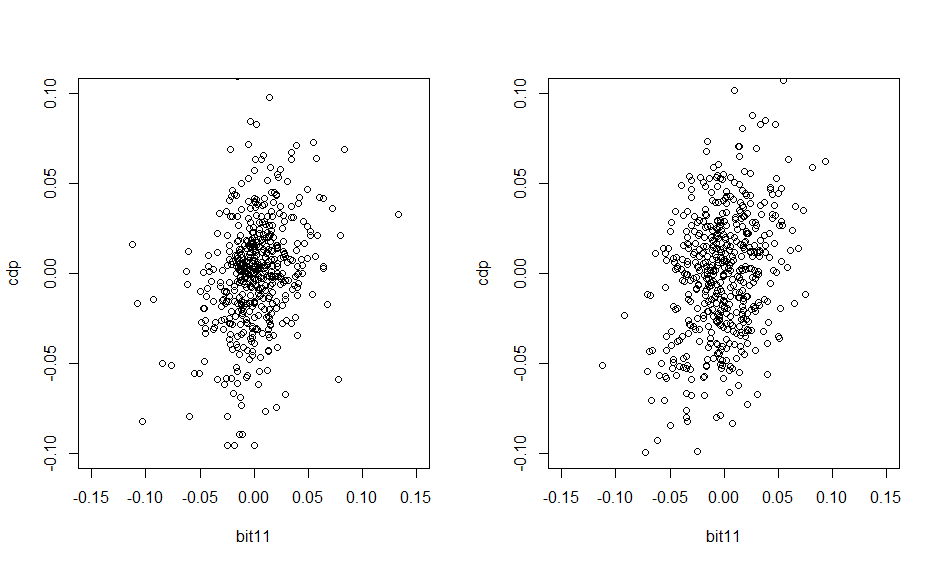
\includegraphics[width=13cm]{Wykresy/QQploty.png}
    \caption{Wykresy rozrzutów: pierwrszy -otrzymany na podstawie danych, drugi - w oparciu o wygenerowaną próbę}
    \label{fig:mlp}
\end{figure}
Po wygenerowaniu próbę liczności danych = 509, na powyższym wykresie widać, że nasze dane nie przypominają rozkładu normalnego. Skupienie danych na obu rozkładach jest rózne. Jest też wiele wartości odstających.
\\ \\
\newpage
Badanie hipotezy mówiącej o tym, że kwadrat odległości Mahalanobisa wektora cen od średniej ma rozkład $\chi^2$ (drugiego stopnia).
\begin{figure}[H]
    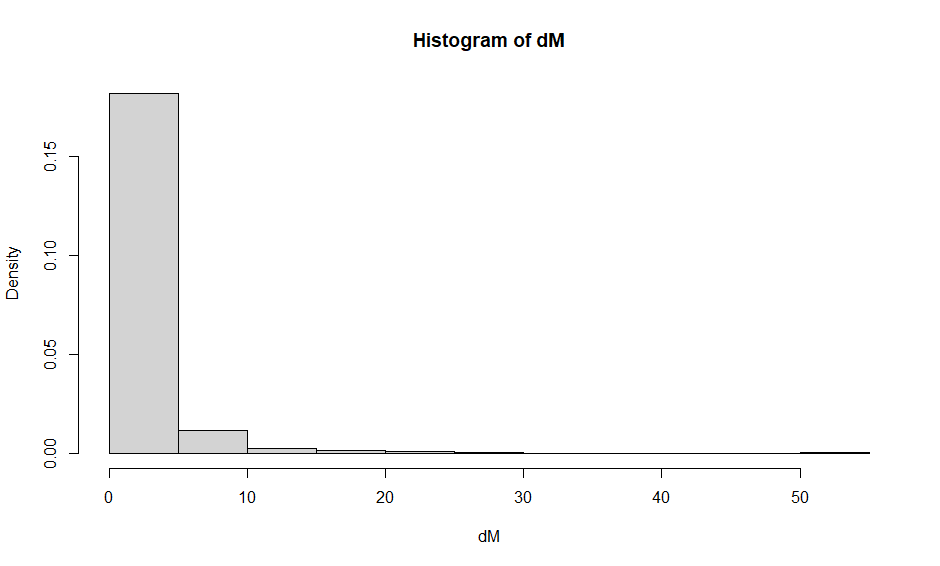
\includegraphics[width=13cm]{Wykresy/Histogram_Mahalanobis.png}
    \caption{Histogram kwadratów odległości Mahalanobisa}
    \label{fig:mlp}
\end{figure}
Zasadnicza większość wartości znajduje się w pierwszym przedziale. Histogram nie ma zbliżonego kształtu do rozkładu $\chi^2$ (drugiego stopnia) -  ma dużą wartość na początku, a następnie bardzo małe, wręcz bliskie zeru (nie jest tak "płynny" jak powinien być).

\begin{figure}[H]
    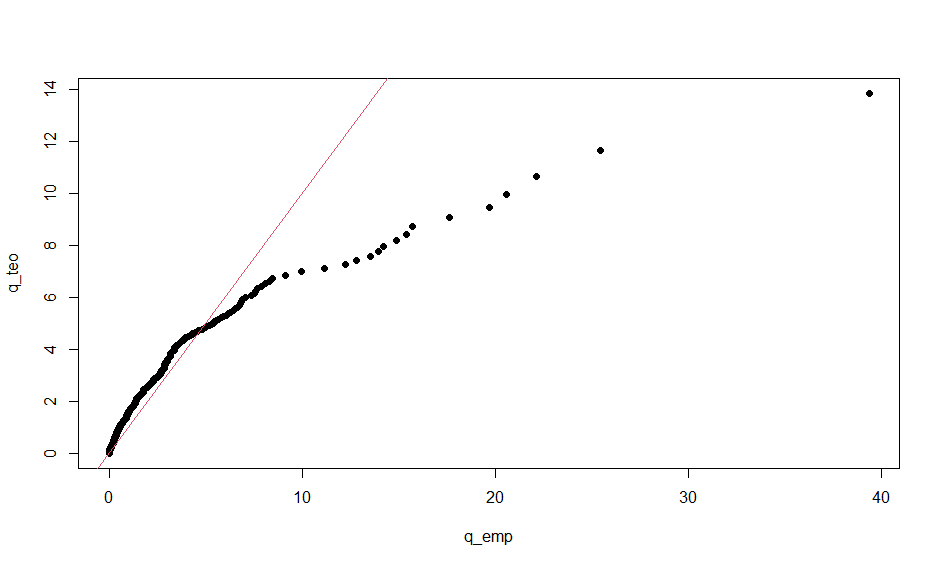
\includegraphics[width=13cm]{Wykresy/QQplot_Mahalanobis.png}
    \caption{Wykres diagnostyczny typu QQ-plot}
    \label{fig:mlp}
\end{figure}

Wykres QQ-plot pokazuje również, iż rozkład $\chi^2$ (drugiego stopnia) nie pasuje do naszych danych. Dane empiryczne początkowo pokładają się z danymi teoretycznymi, lecz szybko zaczynają znacząco od siebie odbiegać.
\\

Po przetestowaniu hipotezy że kwadrat odległości Mahalanobisa wektora cen od średniej maja rozkład $\chi^2$(2) i statystyk Kołmogorowa-Smirnowa, uzyskano wyniki:
  $$ D = 0.16836 $$
  $$ p = 5.882e^{-13} $$ 

Wartość p jest mniejsza od przyjętego poziomu istotności,

   $$ \alpha  = 5\%$$

Zatem hipotezę odrzucamy.


\section{Rozdział 3}
\section{Podsumowanie}
\end{document}

\\ \hline